%!TEX root = main.tex

\section{Index Reduction Algorithm}

\subsection{Working Principle}

\begin{frame}{Index Reduction Algorithm}{Working Principle}
  The index reduction algorithm is based on \textbf{three} steps \dots
  \begin{columns}
    \begin{column}[c]{0.2\textwidth}
      \flushright
      \vspace{-1.25em}%
      \uncover<4->{\begin{tikzpicture}[overlay, remember picture]
        \draw[fg_sl_color, thick, -stealth] (0.5,-1.75) -- (0.0,-1.75) -- (0.0,1.75) -- (0.5,1.75);
        \node[text width=0.75\textwidth, align=center] at (-1.0,0.0) {If $\mE$ is singular};
        %\draw[fg_sl_color, thick, -stealth] (-1.0,-0.5) -- (-1.0,-2.75);
      \end{tikzpicture}}
    \end{column}
    \begin{column}[c]{0.85\textwidth}
      \begin{enumerate}[<+->]
        \item Consider the generic \acsp{DAE} system
        \begin{equation*}
          \mF = \mA \mxp - \mb = \m{0}
        \end{equation*}
        \item \textbf{Separate} the differential and algebraic equations of the system
        \begin{equation*}
          \begin{bmatrix} \mE \\ \m{0} \end{bmatrix} \mxp = \begin{bmatrix} \mg \\ \ma \end{bmatrix}
        \end{equation*}
        \item \textbf{Reduce} the index by differentiating the algebraic equations $\ma = \m{0}$
      \end{enumerate}
    \end{column}
  \end{columns}
  \vspace{0.75em}
  \uncover<5->{This \textbf{repeats} until a \acs{ODE} system with invariants is obtained.}
\end{frame}

\subsubsection{Separation of Differential and Algebraic Equations}

\begin{frame}{Index Reduction Algorithm}{Separation of Differential and Algebraic Equations}
  \vspace{-1.0em}
  \begin{columns}
    \begin{column}[c]{0.6\textwidth}
      \begin{enumerate}[<+->]
        \item Consider the \textbf{generic} \acsp{DAE} system
        \begin{equation*}
          \mF = \mA \mxp - \mb = \m{0}
        \end{equation*}
        \item \textbf{Separate} the equations with the cokernel $\mK$ and its orthogonal complement $\mN$ of $\mE$
        \begin{equation*}
          \begin{bmatrix} \mE \\ \m{0} \end{bmatrix} \mxp = \begin{bmatrix} \mg \\ \ma \end{bmatrix}
          ~~ \text{with} ~~
          \begin{array}{r@{~}c@{~}l}
            \mE &=& \mN \mA \\
            \mg &=& \mN \mb \\
            \ma &=& \mK \mb
          \end{array}
        \end{equation*}
      \end{enumerate}
      \uncover<3->{\begin{bbox}[Cokernel Computation]
        The cokernel $\mK$ and its orthogonal complement $\mN$ of $\mE$ are calculated using \acs{LU} or \acs{FFLU} factorizations.
      \end{bbox}}
    \end{column}
    \begin{column}[c]{0.4\textwidth}
      \visible<3->{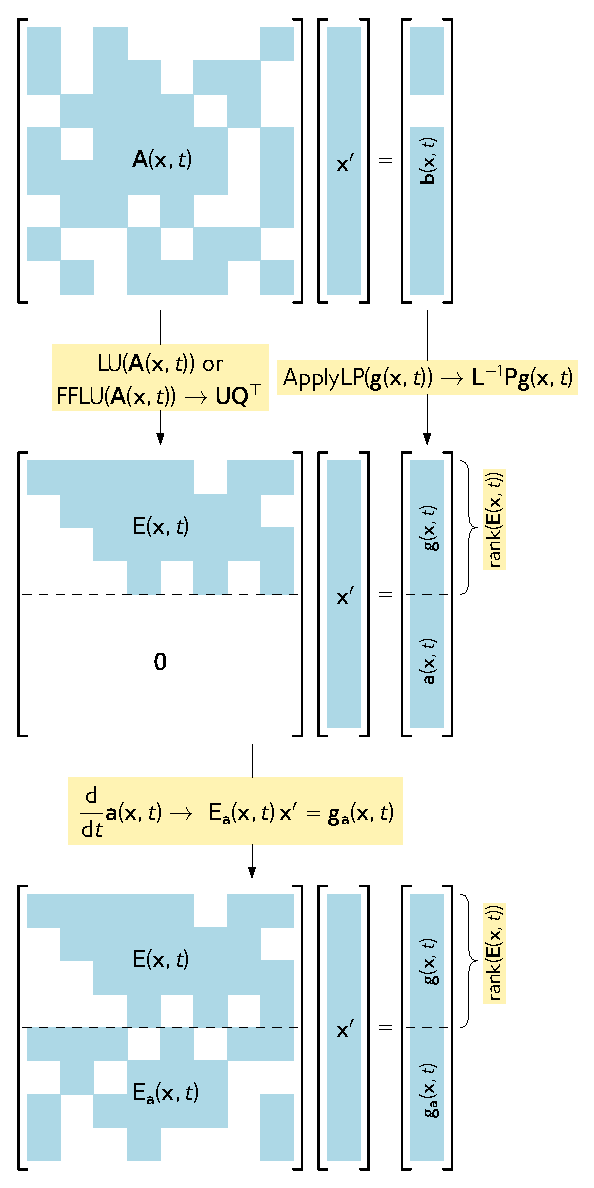
\includegraphics[width=1.0\textwidth, trim={0cm 7.35cm 0cm 0cm}, clip]{dae_visualization.eps}}
    \end{column}
  \end{columns}
\end{frame}

\subsubsection{Differentiation of Algebraic Equations}

\begin{frame}{Index Reduction Algorithm}{Differentiation of Algebraic Equations}
  \vspace{-1.0em}
  \begin{columns}
    \begin{column}[c]{0.6\textwidth}
      \begin{enumerate}[<+->]\setcounter{enumi}{2}
        \item \textbf{Differentiate} the algebraic equations $\ma$
        \begin{equation*}
          \dfrac{\text{d}}{\text{d}t} \ma = \mAd \mxp - \mgd
        \end{equation*}
        \item The new system of \acsp{DAE} takes the form
        \begin{align*}
          \mF = \mA &\mxp - \mb = \m{0} ~~ \text{with} \\
          \mA = \begin{bmatrix} \mE \\ \mAd \end{bmatrix}
          ~~ &\text{and} ~~
          \mb = \begin{bmatrix} \mg \\ \mgd \end{bmatrix}
        \end{align*}
        \item The differential index has been reduced by one!
      \end{enumerate}
      \uncover<4->{\begin{bbox}[A Sequential Algorithm]
        Apply \boxednumber{1}--\boxednumber{5} repeatedly until $\mA$ is non-singular.
      \end{bbox}}
    \end{column}
    \begin{column}[c]{0.4\textwidth}
      \visible<3->{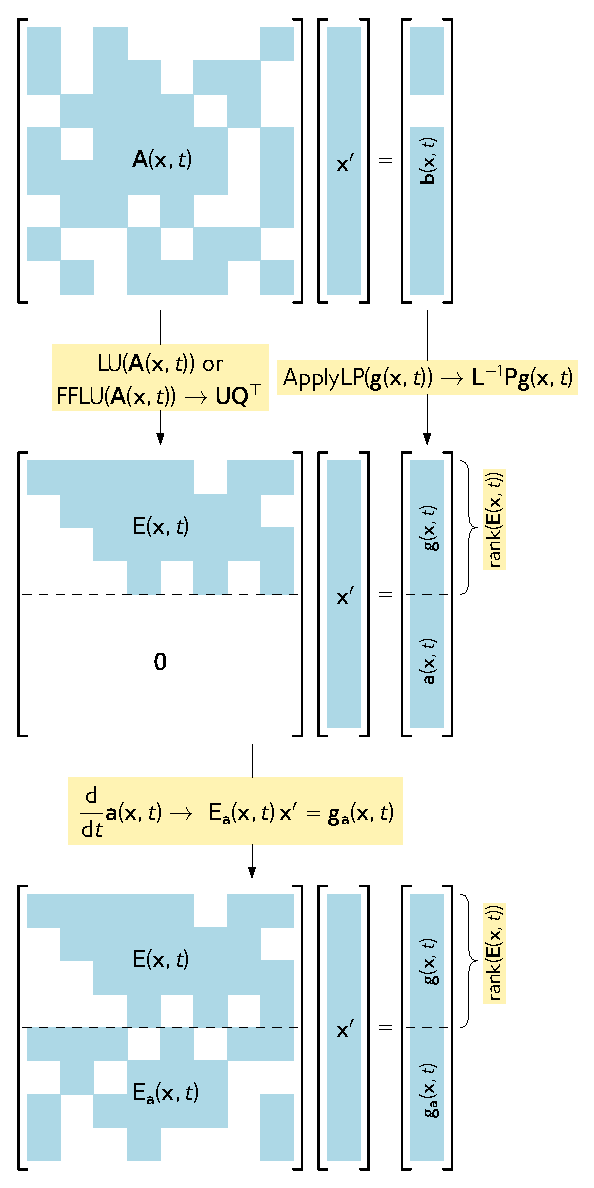
\includegraphics[width=1.0\textwidth, trim={0cm 0cm 0cm 7.35cm}, clip]{dae_visualization.eps}}
    \end{column}
  \end{columns}
\end{frame}

\begin{frame}{Index Reduction Algorithm}{Including Veiling Variables}
  \vspace{-1.0em}
  The algorithm can be extended to include \acs{LEM} \dots
  \begin{itemize}
    \item the veiling variables are stored in the list of $\mv$;
    \item the equations be also function of $\mv$;
    \item the veiling variables do just add an evaluation layer to the algorithm.
  \end{itemize}
  \visible<2->{\vspace{-1.5em}\hspace{-0.025\textwidth}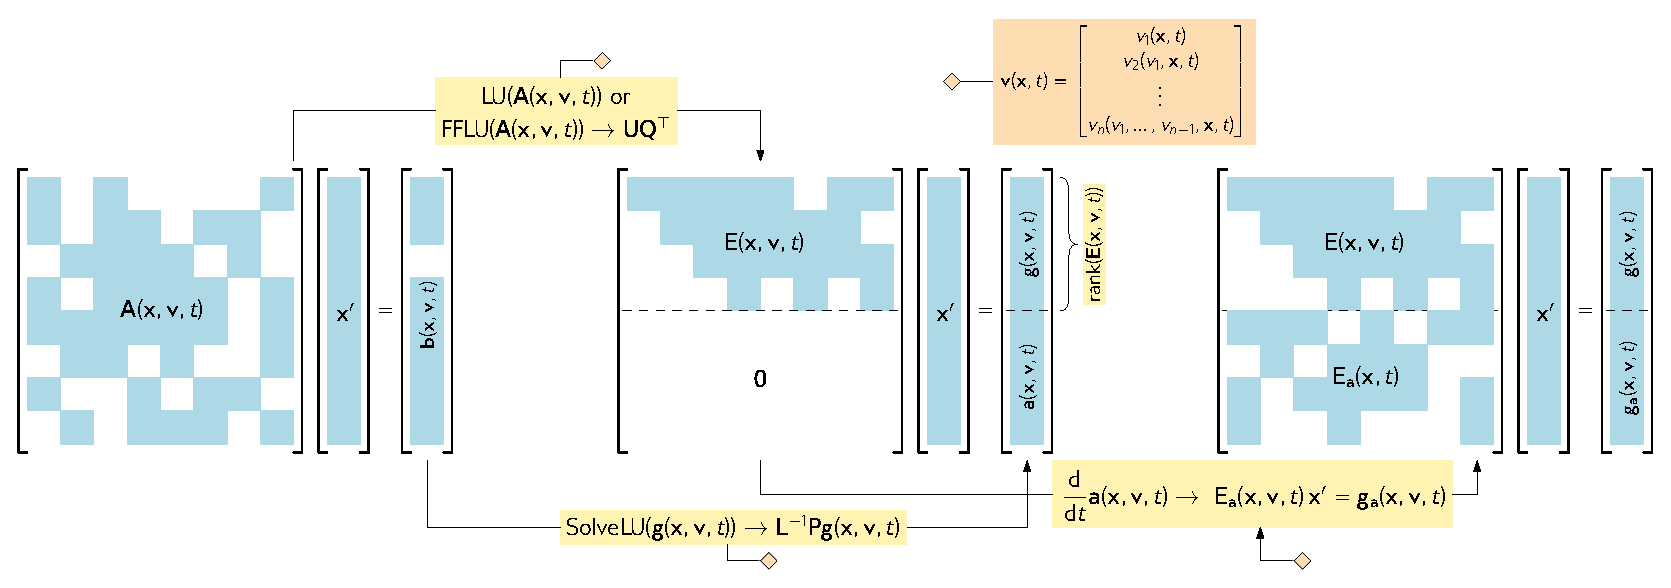
\includegraphics[width=1.05\textwidth]{dae_visualization_veil.eps}}
\end{frame}

\begin{frame}{Index Reduction Algorithm}{Algorithm Flowchart}
  \centering
  \begin{tikzpicture}[overlay]
    \node at (0,0) {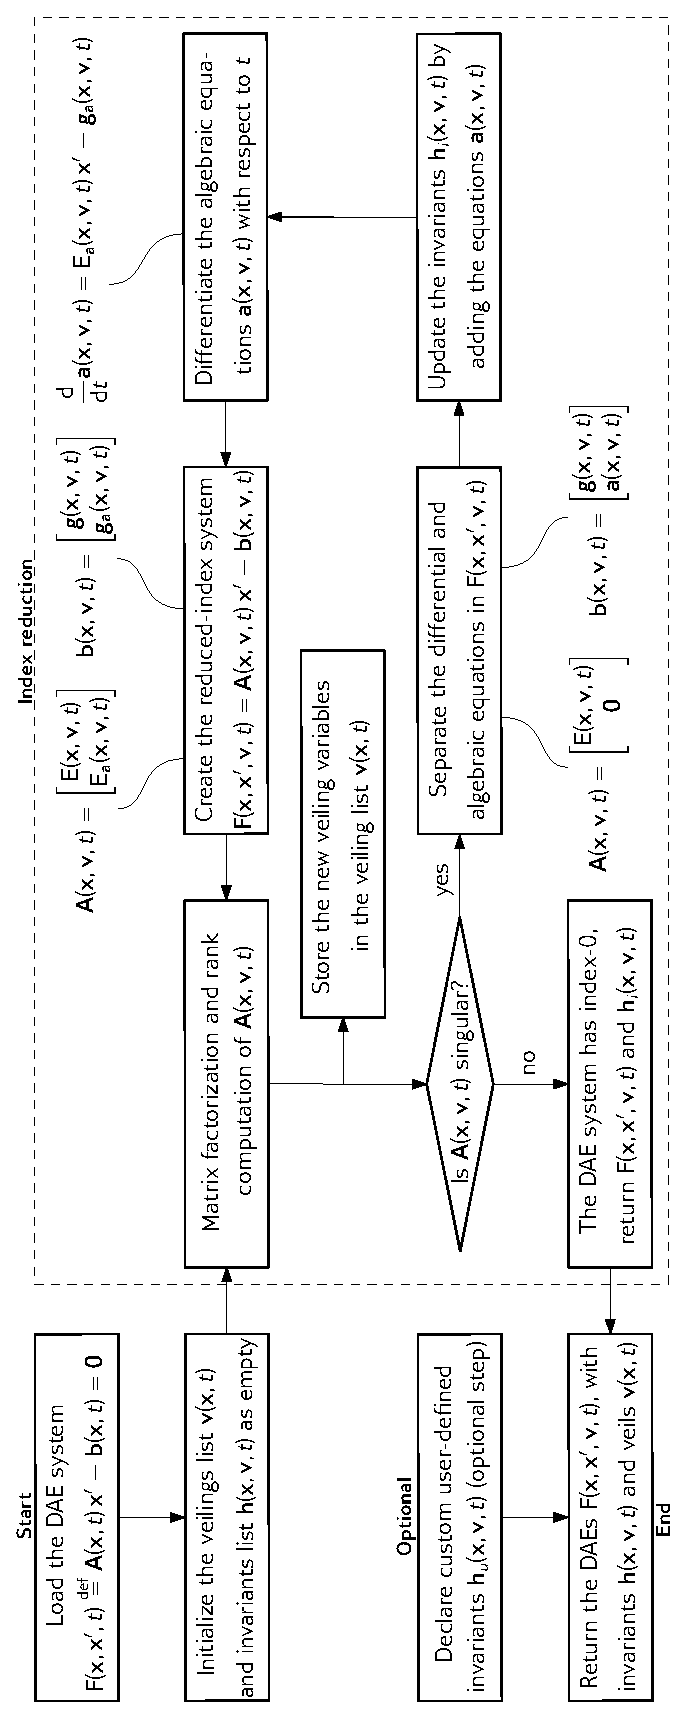
\includegraphics[angle=270, width=1.0\textwidth]{dae_flowchart_veil}};
    \only<1>{\draw[fg_sl_color, line width=1.0pt] (-7.2,  2.9) rectangle (-3.7,  0.4);} % Initialization
    \only<2>{\draw[fg_sl_color, line width=1.0pt] (-3.7,  2.9) rectangle ( 7.2, -2.9);} % Index Reduction
    \only<3>{\draw[fg_sl_color, dashed, line width=1.0pt] (-7.2, -0.3) rectangle (-3.7, -1.6);} % Optional step
    \only<4>{\draw[fg_sl_color, line width=1.0pt] (-7.2, -1.6) rectangle (-3.7, -2.9);} % Finalization
  \end{tikzpicture}
\end{frame}

\begin{frame}{Index Reduction Algorithm}{The Reduced \acs{DAE} System}
  The index-reduced system of \acsp{DAE} takes the form \dots
  \begin{itemize}[<+->]
    \item \textbf{Differential part}
    %
    \begin{equation*}
      \begin{array}{ccl}
          \m{F}(\mx, \mx^\prime, \m{v}, t) = \m{0} & \quad & \text{implicit  system class} \\
          \m{A}(\mx, \m{v}, t) \mx^\prime = \m{b}(\mx, \m{v}, t) & \quad & \text{semi-explicit system class} \\
          \mx^\prime = \m{f}(\mx, \m{v}, t) & \quad & \text{explicit system class}
      \end{array}
    \end{equation*}
    %
    \item \textbf{Invariants}
    %
    \begin{equation*}
      \m{h}(\mx, \m{v}, t) = \begin{bmatrix}
          \mhiv \\
          \mhuv
      \end{bmatrix} = \m{0} \quad \begin{array}{l}
        \text{hidden constraints} \\
        \text{\emph{optional} user-defined invariants}
        \end{array}
    \end{equation*}
    %
    \item \textbf{Veiling variables}
    %
    \begin{equation*}
        \m{v}(\mx, t) = \begin{bmatrix}
            v_{1}(\mx, t) \\
            v_{2}(v_{1}, \mx, t) \\
            \vdots \\
            v_{n}(v_{1}, \dots, v_{n-1}, \mx, t)
        \end{bmatrix}
    \end{equation*}
  \end{itemize}
\end{frame}

\subsection{Projection on Invariants}

\begin{frame}{Projection on Invariants}{Theoretical Background and Implementation}
  \begin{columns}
    \begin{column}[c]{0.6\textwidth}
      Projection is performed \dots
      \begin{itemize}
        \item during the \textbf{numerical integration}
        \item to \textbf{enforce} the solution $\mx$ onto the $\mhv$ manifold
        \item by solving the \textbf{constrained minimization} problem
          \begin{align*}
            \underset{\mx}{\text{minimize}} \quad &\dfrac{1}{2}\left(\mx - \tilde{\mx}\right)^2 \\
            \text{subject to} \quad &\mhv = \m{0}
          \end{align*}
        \end{itemize}
      \end{column}
      \begin{column}[c]{0.4\textwidth}
        \hspace{-0.2\textwidth}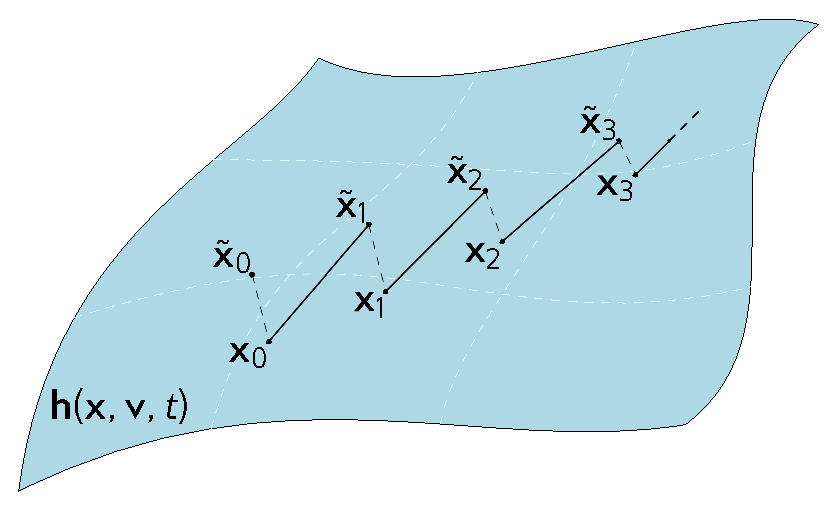
\includegraphics[width=1.2\textwidth]{projection.eps}
      \end{column}
    \end{columns}
    \vspace{1.0em}
    \hic{\large Find $\mx$ with minimal distance from $\tilde{\mx}$ that satisfies the invariants $\mhv$}
\end{frame}

\begin{frame}{Projection on Invariants}{Theoretical Background and Implementation}
  \begin{itemize}
    \item The \textbf{Lagrangian} of the minimization problem is
    \begin{equation*}
      \mathcal{L}(\mx, \boldsymbol{\lambda}) = \frac{1}{2}\left(\mx - \tilde{\mx}\right)^2 + \boldsymbol{\lambda} \cdot \mhv
      \quad \rightarrow \quad
      \begin{cases}
        \mx + \m{Jh}_\mx^\top \boldsymbol{\lambda} = \tilde{\mx} \\
        \mhv = \m{0}
      \end{cases}
    \end{equation*}
    \item The problem is solved using the iterative method
    \begin{equation*}
      \begin{bmatrix}
        \m{I}        & \m{Jh}_\mx^\top \\
        \m{Jh}_{\mx} & \m{0}
      \end{bmatrix}
      \begin{bmatrix}
        \delta\mx \\
        \boldsymbol{\lambda}
      \end{bmatrix} = \begin{bmatrix}
        \tilde{\mx} - \mx \\
        -\mhv
      \end{bmatrix} \quad \text{where the step is} \quad \mx = \tilde{\mx} + \delta\mx
    \end{equation*}
    \item[] \dots derived from the \textbf{Taylor expansion}
    \begin{equation*}
      \begin{cases}
        \mhv + \m{Jh}_{\mx}(\mx, \m{v}, t) \delta\mx + \textcolor{mycolor2}{\mathcal{O}\left(\| \delta\mx \|^2\right)} = \m{0} \\
        \mx + \delta\mx + \m{Jh}_{\mx}^{\top}(\mx + \textcolor{mycolor2}{\delta \mx}, \m{v}, t) \boldsymbol{\lambda} = \tilde{\mx}
      \end{cases}
    \end{equation*}
  \end{itemize}
\end{frame}

\begin{frame}{Symbolic-Numerical Validation}{The Problem}
  \begin{columns}
    \begin{column}[t]{0.425\textwidth}
      A \textbf{particle} moving over a \textbf{torus} surface% on a \textbf{stable path}
      \begin{equation*}
        \label{chap4:eq:torus}
        \begin{cases}
          x^{\prime}_{1} = u_{1} \\
          x^{\prime}_{2} = u_{2} \\
          x^{\prime}_{3} = u_{3} \\
          u^{\prime}_{1} = u_{3}\cos(t) - x_{3}\sin(t) - u_{2} + 2 c x_{1}\lambda \\
          u^{\prime}_{2} = u_{3}\sin(t) + x_{3}\cos(t) + u_{1} + 2 c x_{2}\lambda \\
          u^{\prime}_{3} = x_{3} + 2x_{3}\lambda \\[-0.1em]
          \rho^2 = x_{1}^2 + x_{2}^2 + x_{3}^2 - 2r\sqrt{x_{1}^2 + x_{2}^2} + r^2
        \end{cases}
      \end{equation*}
      with $c = 1 - \dfrac{r}{\sqrt{x_{1}^2 + x_{2}^2}}$.
    \end{column}
    \begin{column}[t]{0.575\textwidth}
      \vspace{-4.0em}
      \hic{\large A stable path \dots}
      with $\mx_{0} = [15, 0, 0, 0, 15, -5, \lambda]^{\top}$ and parameters $\rho = 5$ and $r = 10$ is given by
      \begin{equation*}
        \mx_\text{exact} = \begin{bmatrix}
          x_{1} \\ x_{2} \\ x_{3}
        \end{bmatrix} = \begin{bmatrix}
          (\rho \cos(2\pi - t) + r) \cos(t) \\
          (\rho \cos(2\pi - t) + r) \sin(t) \\
          \rho \sin(2\pi - t)
        \end{bmatrix}
      \end{equation*} \\[-3.0em]
      \centering{
      \begin{tikzpicture}
        \begin{axis}[
          xtick=\empty, ytick=\empty, ztick=\empty,
          axis line style={draw=none},
          tick style={draw=none},
          axis equal,
          view={100}{40}]
          \addplot3[surf,
            samples=50,
            color=mycolor1, opacity=0.25,
            faceted color=mycolor1!20,
            domain=0:2*pi,
            y domain=0:2*pi,
            z buffer=sort]
            ({(10+5*cos(deg(x)))*cos(deg(y+pi/2))},
              {(10+5*cos(deg(x)))*sin(deg(y+pi/2))},
              {5*sin(deg(x))});
          \addplot3[variable=\t,
            no markers,
            samples=50,
            color=mycolor4,
            domain=0:2*pi,
            line width=0.5pt]
            ({(10+5*cos(deg(2*pi-\t)))*cos(deg(\t))},
              {(10+5*cos(deg(2*pi-\t)))*sin(deg(\t))},
              {5*sin(deg(2*pi-\t))});
          %\addplot3[
          %  mark=*, mark size=1.0pt,
          %  color=mycolor4]
          %  ({(10+5*cos(deg(2*pi-0.1*pi)))*cos(deg(0.1*pi))},
          %    {(10+5*cos(deg(2*pi-0.1*pi)))*sin(deg(0.1*pi))},
          %    {5*sin(deg(2*pi-0.1*pi))});
        \end{axis}
      \end{tikzpicture}}
    \end{column}
  \end{columns}
\end{frame}

\begin{frame}{Symbolic-Numerical Validation}{Order and Error Analysis}
  \vspace{-1.0em}
  \hic{The order and the invariants are preserved}
  \centering{\small{\input{figures/torus_order_hidden.tex}}}
\end{frame}

\begin{frame}{Symbolic-Numerical Validation}{Solution Visualization}
  \begin{columns}
    \begin{column}[c]{0.22\textwidth}
      \hic{\large The importance of projection \dots}
      $\Delta t = 0.05$\,s \\ $t \in [0, 200\pi]$\,s
    \end{column}
    \begin{column}[c]{0.77\textwidth}
      \centering\small
      \textbf{RadauIIA5 - No projection}%
      \hspace{3.5em}%
      \textbf{RadauIIA5 - With projection}
      \movie[label=show1, width=0.95\textwidth, autostart, poster, showcontrols, loop]{\includegraphics[width=0.95\textwidth]{torus_3d_placeholder.png}}{movie/torus_3d.mov}
    \end{column}
  \end{columns}
\end{frame}

% That's all Folks!